The original hypothesis of this research was that "\textit{Individual and population level air pollutant exposure can be estimated using time-activity surveys, \gls{gis} and routing tools, and then coupled with high resolution spatio-temporal air quality models to facilitate a greater understanding of the health impacts of air pollution and how public health risks can be reduced}". This was expanded with the following objectives:

\begin{enumerate}
\item Reconstruct the time-space activity of London's population
\item Link modelled air quality, estimate exposure, and compare with traditional methods
\item Refine the models estimates of London Underground exposure
\item Evaluate the results
\end{enumerate}

This research has gone a long way to proving this hypothesis through the creation of a tool that allows scientists to examine individual-level and group exposure to ranges of pollutants in a range of microenvironments. The chapters on '\nameref{chap:the_ltdsx}' (Chapter \ref{chap:the_ltdsx}) and '\nameref{chap:the_lhem}' (Chapter \ref{chap:the_lhem}), which were the main chapters centred around the creation of the tool, have been published as \cite{Smith2016} (the model development and use), and then subsequently used by \cite{Tonne2018} to examine socioeconomic and ethnic inequalities in exposure to poor air quality.

The chapter '\nameref{chap:monitoring_on_underground}' (Chapter \ref{chap:monitoring_on_underground}), on refining the exposure estimates for users of the London Underground after this micro-environment was found to be so important to Londoners exposure, is in the process of being written-up as an academic paper and will provide an open-source dataset ('TubeAir') for calculating the exposure of London Underground users within other studies, or as a stand-alone policy tool (probably for use by TfL and their contractors).

Finally the chapter on '\nameref{chap:evaluating_dynamic_exposure_models}' (Chapter \ref{chap:evaluating_dynamic_exposure_models}), on how to evaluate exposure models of this kind, diverted away from the main hypothesis of the research, but during the previous chapters the reliability and how representative the results are became of interest and importance to consider, and so this seemed necessary. This final chapter concluded by finding that depending on the level of confidence and margin of error, large numbers of personal monitoring data are required to evaluate dynamic models.

%%%%%%%%%%%%%%%%%%%%%%%%%%%%%%%%
\newpage
\section{Discussion}
\label{sec:wrap_up_discussion}
%%%%%%%%%%%%%%%%%%%%%%%%%%%%%%%%

%% Discussion on LTDS-X
\subsection{The LTDS-X}
\label{ltds_discussion_wrapup}


The '\nameref{chap:evaluating_dynamic_exposure_models}' (Chapter \ref{chap:the_ltdsx}) demonstrated how a dataset that was originally purposed for assessing transport demand in London could be adapted, processed and re-purposed to create the \gls{ltds}-X, a high resolution spatial and temporal time-activity dataset (including demographics), that is representative of the daily movements of the population of London. The main limitation with using this dataset as an input to the exposure modelling, were that the data were London-centric, and 'porting' this method to another city or country would require a similar or replacement dataset. Though as the model is mechanistic rather than empirical, theoretically this should be possible. Whilst undertaking this research other datasets have been investigated and considered as substitutes for the \gls{ltds}, for example in the 2011 UK Census, a new question of 'workplace zones' was asked of the population, and research by Dr Reis (Centre for Ecology and Hydrology, \gls{uk}) is using the responses as a way to model population-level movement for exposure modelling. Using this as a basis, travel exposure from workplace zone to workplace zone by each mode of transport could be simulated and the exposure calculated, and then an indoor exposure module 'plugged-in' to create a UK-wide exposure model. The spatial and temporal detail would not be as high as the \gls{ltds}-X and \gls{lhem}, but the coverage would be much larger. Given Census' are common in many countries around the world, this could be replicated in other places given time and processing. Other datasets such as location data from storecards, credit cards and Twitter could also be incorporated to refine the model.

It is worth noting that whilst this dataset was specifically re-purposed for use as an input to air quality exposure modelling, it could similarly be used for exposure to other things such as perhaps ultra-violet light and risks of skin-cancer, or to estimate where the population are drinking water and therefore links between poor quality water and health. Any type of model that requires human time-activity as an input.

Away from exposure the dataset has been useful in areas of work that the Environmental Research Group is involved in. In 2012 it was used to look at the number of cross-Borough car trips being undertaken as part of the London Atmospheric Emissions Inventory (\gls{laei}), and in 2018 was used to identify whether active travel has increased or decreased in the London Borough of Waltham Forest as part of a contract piece of work.\\

%% Discussion on dynamic exposure
\subsection{Dynamic exposure}
\label{dynamic_exposure_wrapup}

In the chapter on '\nameref{chap:the_lhem}' (Chapter \ref{chap:the_lhem}), having built the \gls{ltds}-X, this was combined with \gls{cmaq}-UK and microenvironmental modelling methods to quantify at unprecedented detail the exposure of the London population to poor air quality (The \gls{lhem}). The size, detail and possibilities for future research of this model were demonstrated by focusing on exposure missclassification, and this work was published in \cite{Smith2016} . The applications for this model are already being taken forward in other exposure studies, including the project 'CLUE II' led by Imperial College London looking at the air quality and noise exposure of children in London, and the COPE (Characterisation of \gls{copd} Exacerbations using Environmental Exposure Modelling) study led by \gls{kcl}. As was highlighted in the Chapter, it is our hope that this type of tool can increasingly be used for policy applications by the likes of \gls{tfl} and the Greater London Authority (\gls{gla}) to better understand the effects of policy interventions on exposure. Indeed, Waltham Forest are using it to investigate the effects on cyclist exposure of introducing segregated cycle lanes, and we are collecting data on behalf of TfL to quantify changes in bus passenger exposure following retrofitting of cleaner engines.

The areas of the \gls{lhem} model that were identified as most in need of improvement were the modelling within microenvironments, which included time in enclosed transport (bus, car, train, tube), and time indoors. There are a number of studies that consider these microenvironments, but the results are highly variable. Similarly, little was known about the exposure of passengers on the London Underground while making the \gls{lhem}. When the initial \gls{lhem} results were being analysed it transpired that this was an important determinant of high daily exposures in the population, and therefore the objectives/research plan for the following chapter were developed.\\

%% Discussion on tube exposure
\subsection{The London Underground}
\label{london_underground_wrapup}

The chapter '\nameref{chap:monitoring_on_underground}' (Chapter \ref{chap:monitoring_on_underground}) involved an extensive mobile monitoring campaign on the London Underground, and creation of a dataset for estimating \gls{pm25} passenger exposure during journeys on the network. Other research has been undertaken in the London Underground, but not to this spatial coverage, not geographically referenced, and not made publicly available. That is not to say it cannot be improved; there are a small number of stations that are not yet mapped, and specifically stations with multiple lines need further sampling and data refinement to separate these into different exposure estimates. Also further sampling could be undertaken to establish the repeatability of concentrations. This research has directly led to a sub-group of \gls{comeap} being formed, and a report on "available evidence on the health risks associated with particulate matter exposure in the London Underground" being written, aswell as \gls{tfl} commissioning further monitoring on station platforms.

Within the Environmental Research Group at \gls{kcl}, Dr Green has also been contracted by \gls{tfl} to undertake further monitoring on station platforms. The data and research should be published later in 2018 which is expected to lead to further opportunities and incorporation into other studies. For example the exposure tool was used to create an origin-destination matrix of exposure between stations on the Northern Line of the London Underground, shown in Figure \ref{fig:time_weighted_tube_exposure} below .

\begin{figure}[H]
\centering
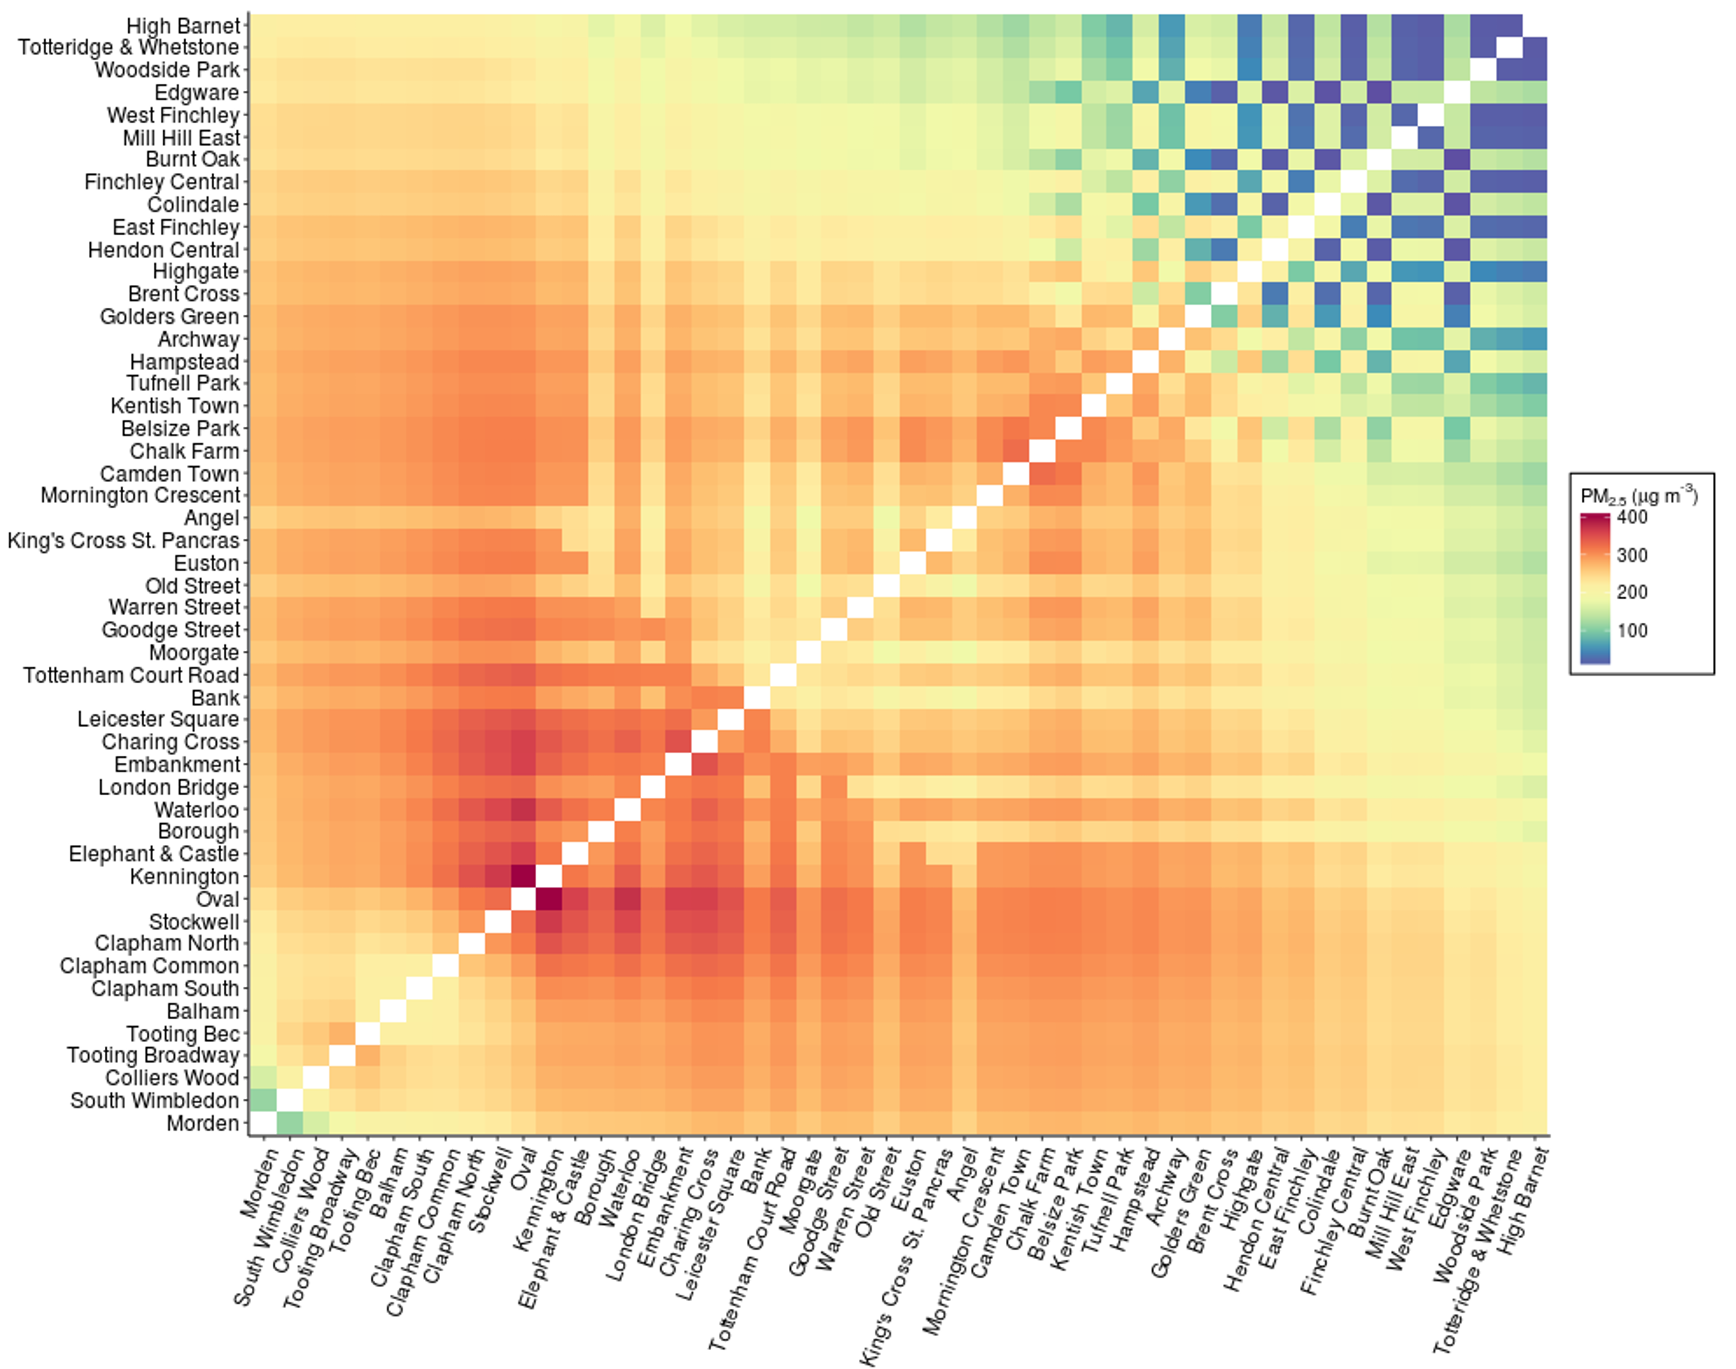
\includegraphics[scale=0.6]{images/time_weighted_tube_exposure}
\caption{Time-weighted exposure between tube stations on the Northern Line}
\label{fig:time_weighted_tube_exposure}
\end{figure}

%% Discussion on evaluation
\subsection{Evaluating dynamic exposure models}
\label{evaluation_wrapup}

The area of research in the chapter on '\nameref{chap:evaluating_dynamic_exposure_models}', has been poorly addressed in publications in this area. It is common for authors to comment on the accuracy of their outdoor air quality model, how representative the microenvironmental modelling is, the quality of the time-activity data, or other such factors. But not to consider how to combine these factors, and not how to undertake sampling of journeys for comparison. The chapter on '\nameref{chap:evaluating_dynamic_exposure_models}' (Chapter \ref{chap:evaluating_dynamic_exposure_models}) doesn't solve this problem, but demonstrates the issues and takes a first step at addressing one of them; how many samples of air quality are needed to be representative of annual averages across a journey (and the issues with collecting this data). It lends weight to the 'distributed sensor network' notion that has been mooted in publications such as \cite{Moltchanov2015} and \cite{Broday2017}, and how these could be useful in exposure science rather than simply as a new type of monitoring site. By taking continuous mobile measurements all over a city, for example on all buses and bike-hire schemes, these repeat samples could be aggregated and a better understanding of hyper-local air quality developed to evaluate air quality modelling (and exposure).

%%%%%%%%%%%%%%%%%%%%%%%%%%%%%%%%
\newpage
\section{Conclusions}
\label{sec:wrap_up_conclusions}
%%%%%%%%%%%%%%%%%%%%%%%%%%%%%%%%

\subsection{Modelling Londoners movements}
\label{subsec:wrapup_conc_ltds}

\begin{itemize}
    \item While there are clear peaks in the morning and evening, there is substantial travel in London outside of peak hours
    \item Men tend to travel longer distances than women each day
    \item As household income increases, daily travel distance increases
    \item Travel distance increases with age, peaking around 40, then declines.
    \item The very old ($>$80) tend to only take short journeys over small distances.
    \item People over 80 rarely use the London Underground
    \item Between 20 and 50 years old, people spend about 70\% of their time within 1km of their home.
\end{itemize}

\subsection{Dynamic exposure modelling}
\label{subsec:wrapup_conc_exposure}

\begin{itemize}
    \item Londoners are exposed to 85\% of their daily \gls{no2} and 90\% of their daily \gls{pm25} while indoors
    \item Increasing active travel results in daily lower exposure to both pollutants.
    \item Epi studies are likely overestimating exposure when using address point concentrations.
    \item There seems to be little difference between postcode and address-point exposure estimates
    \item Exposure missclassification increases in relation to the amount of travel that people undertake, especially inactive travel
    \item Londoners are exposed to peaks of unacceptable (according to the WHO) \gls{pm25} and \gls{no2} levels for between 13-16\% and 1-4\% of their day, depending on age group.
    \item \gls{pm25} and \gls{no2} exposure is correlated at the address level, but not in a dynamic exposure model.
\end{itemize}

\subsection{Exposure to \texorpdfstring{\gls{pm25}}{} on the London Underground}
\label{subsec:wrapup_conc_underground}

\begin{itemize}
    \item \gls{pm25} concentrations on the London Underground vary between 0 $\mu \text{g m}^{-3}$ and 990 $\mu \text{g m}^{-3}$, with a mean of 129 $\mu \text{g m}^{-3}$.
    \item There are large variations between lines, and between sections of track on the same line.
    \item When ranked in decreasing order of mean \gls{pm25} concentrations, London Underground lines have the following concentrations:
\end{itemize}

\definecolor{victoria}{rgb}{0,0.711,0.882}
\definecolor{northern}{rgb}{0,0,0}
\definecolor{piccadilly}{rgb}{0,0.098,0.658}
\definecolor{bakerloo}{rgb}{0.537,0.027,0.141}
\definecolor{central}{rgb}{0.863,0.141,0.1216}
\definecolor{jubilee}{rgb}{0.525,0.561,0.596117}
\definecolor{metropolitan}{rgb}{0.459,0.063,0.34}
\definecolor{circle}{rgb}{1,0.808,0}
\definecolor{district}{rgb}{0,0.447,0.161}
\definecolor{hammersmithcity}{rgb}{0.843,0.6,0.686}
\definecolor{dlr}{rgb}{0,0.686,0.678}

\begin{table}[H]
\centering
    \begin{tabular}{ | l | l |} \hline
     \cellcolor{victoria} \textcolor{white}{Victoria}                      & 436 $\mu \text{g m}^{-3}$   \\ \hline
     \cellcolor{northern} \textcolor{white}{Northern}                      & 219 $\mu \text{g m}^{-3}$   \\ \hline
     \cellcolor{piccadilly} \textcolor{white}{Piccadilly}                  & 199 $\mu \text{g m}^{-3}$   \\ \hline
     \cellcolor{bakerloo} \textcolor{white}{Bakerloo}                      & 164 $\mu \text{g m}^{-3}$   \\ \hline
     \cellcolor{central} \textcolor{white}{Central}                        & 119 $\mu \text{g m}^{-3}$   \\ \hline
     \cellcolor{jubilee} \textcolor{white}{Jubilee}                        & 115 $\mu \text{g m}^{-3}$   \\ \hline
     \cellcolor{metropolitan} \textcolor{white}{Metropolitan }             & 67 $\mu \text{g m}^{-3}$    \\ \hline
     \cellcolor{circle} \textcolor{white}{Circle}                          & 41 $\mu \text{g m}^{-3}$    \\ \hline
     \cellcolor{district} \textcolor{white}{District}                      & 40 $\mu \text{g m}^{-3}$    \\ \hline
     \cellcolor{hammersmithcity} \textcolor{white}{Hammersmith \& City}    & 36 $\mu \text{g m}^{-3}$    \\ \hline
     \cellcolor{dlr} \textcolor{white}{DLR}                                & 18 $\mu \text{g m}^{-3}$    \\ \hline
    \end{tabular}
\label{tab:london_underground_air_quality}
\end{table}

\subsection{Evaluating dynamic exposure models}
\label{subsec:wrapup_conc_evaluation}

\begin{itemize}
    \item Evaluating dynamic exposure models requires expertise in personal monitoring, uncertainty analysis, statistics, air quality modelling and geographic information sciences.
    \item For 20m by 20m modelled air quality representing one hour in August and September, it was estimated around 540 measurements would be required in each grid square to give a 90\% confidence with 10\% margin of error.
    \item As temporal resolution of air quality models increase, the number of samples to evaluate the data increases.
    \item \gls{cmaq}-UK appears to be under estimating air quality concentrations (and therefore exposure) on the route chosen for evaluation
\end{itemize}

%%%%%%%%%%%%%%%%%%%%%%%%%%%%%%%%
\newpage
\section{Future work}
\label{sec:future_work}
%%%%%%%%%%%%%%%%%%%%%%%%%%%%%%%%

The natural direction of dynamic exposure modelling of this kind is to expand the geographical coverage, increase the numbers of subjects, the accuracy of the modelling (both in terms of the exposure predictions and how representative of populations the results are), and to then apply the model to human health studies. There are also a number of methodological ways that the model could be improved which will enable the model to be used quicker and more effectively. These concepts are explored below.

\subsection{Routing improvements}
\label{subsec:routing_improvements}

The creation of the \gls{ltds}-X in Chapter \ref{chap:the_ltdsx} was mostly a result of cleaning of survey data, loading into database software, and then using the PL/R PostgreSQL language to communicate between the database and the routing \gls{api}'s through an R interface (with some further data cleaning and processing after this). Whilst this worked, it took a long time to run due to queries failing, and code needing to be re-written to anticipate and deal with various errors elegantly. Other issues included limits on \gls{api} use meaning queries had to be submitted with pauses inbetween them to purposefully slow down the requests. Going forward this should be turned into stand-alone R code, that queries a range of \gls{api}s depending on the rate limits and transport mode, and ideally queries it's own routing server (such as OpenStreetMap (\gls{osm}) where no limits would be enforced. Dr Beddows (who works in the Environmental Research group) and I in our group are currently looking into setting up an ERG-OSM server. Not specifically for use by a hybrid exposure model, but as a general all-purpose tool for geographical datasets. Some of the routing code used in the \gls{lhem} was turned into a stand-alone routing/exposure tool for individual journeys. An R function was created whereby London start and end coordinates could be entered, and a PDF output of exposure on that journey created (Example shown in Figure \ref{fig:exposure_result}).

\begin{figure}[H]
\centering
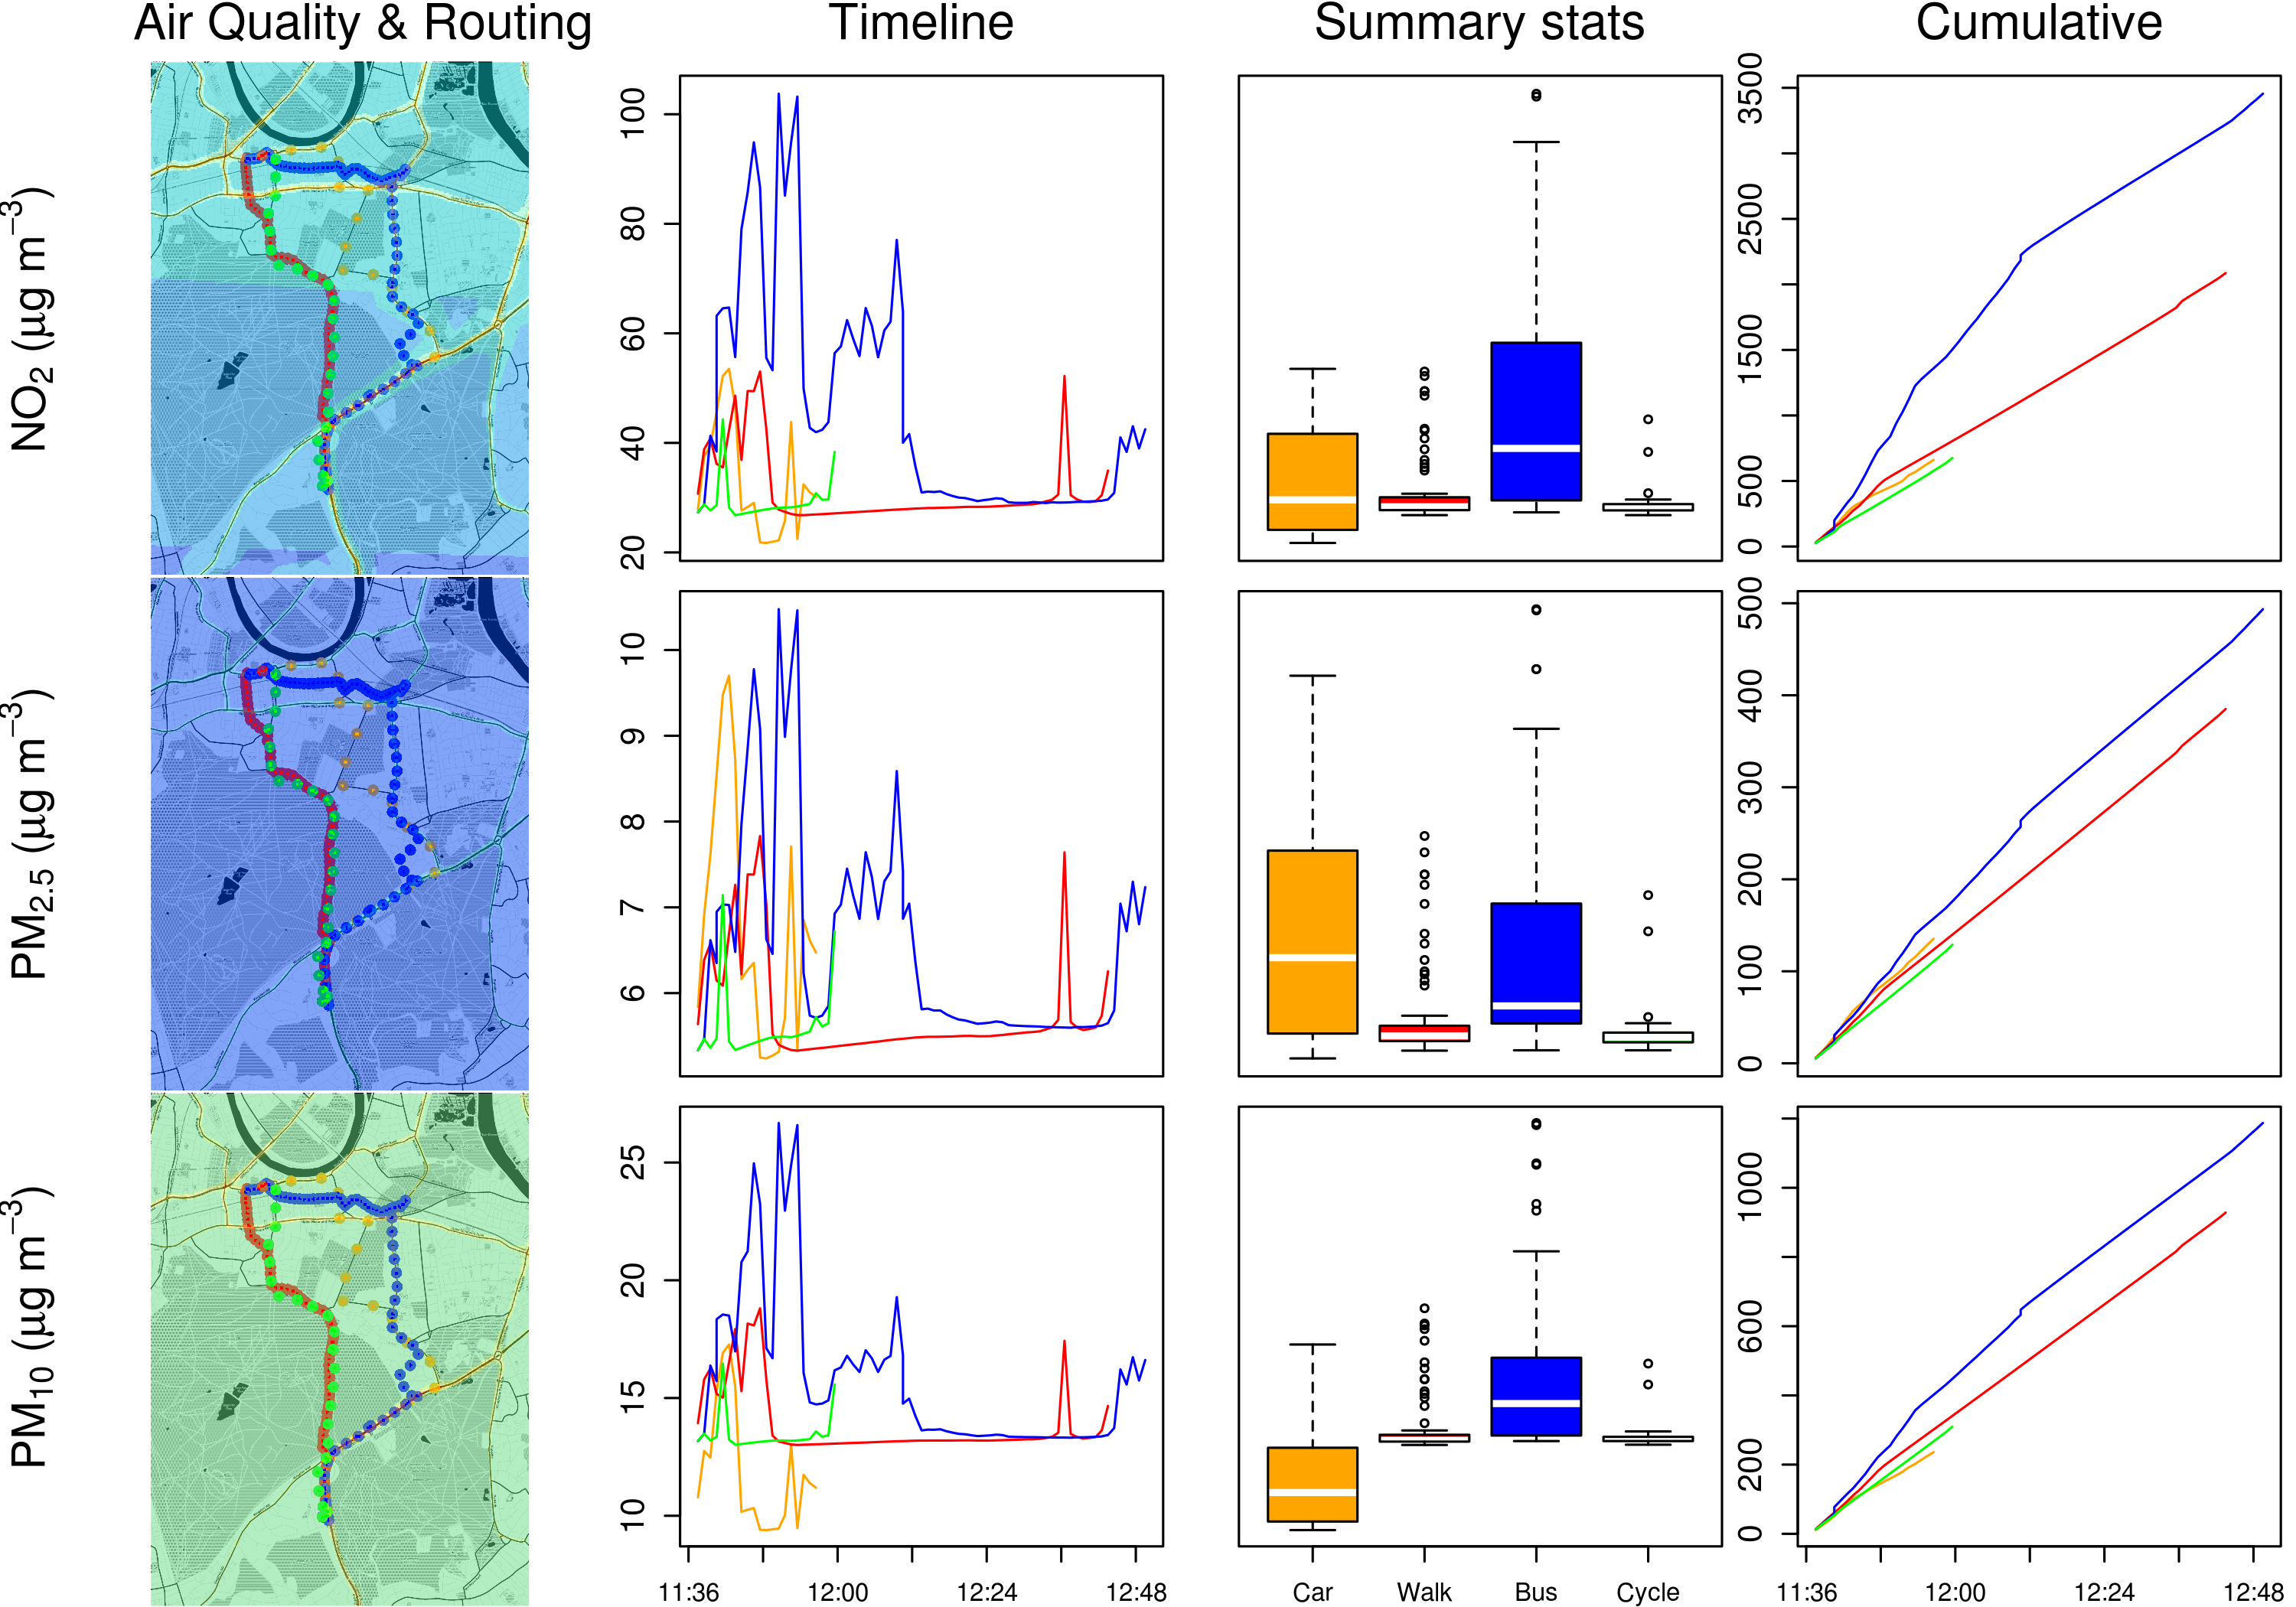
\includegraphics[scale=0.6]{exposure_result.png}
\caption{Example of stand-alone routing tool developed for Drayson}
\label{fig:exposure_result}
\end{figure}

Many of the routing functions that have been created could be considered for adding to a stand-alone R library or package, either newly developed or to an existing package such as 'dodgr' (\cite{dodgr2018}) or 'stplanr' (\cite{strplanr2018}). 

\subsection{Geographical and temporal coverage}
\label{subsec:geographical_coverage}

A logical step for this model is to expand it's geographical coverage, and to incorporate larger numbers of subjects. The \gls{ltds} survey used in this research covered the years 2008 to 2010. However there is now data available from \gls{tfl} up to 2016. In addition, \gls{tfl} have re-calculated the way in which they use scaling factors to represent the population, meaning that longitudinal analysis between years is now possible, such as calculating how cyclists in London's exposure has improved between 2008 and 2016 (providing air quality data for each year is available). Outside of London, using \gls{uk} census data to increase subject coverage would also be desirable, perhaps as a complimentary dataset to the \gls{ltds}, rather than as a replacement. By combining the two, modelling of exposure would be detailed in cities where higher resolution datasets are available, and less detailed where it is not, in a similar way to some of the \gls{cmaq}-UK air quality modelling.

\subsection{Application in health studies}
\label{subsec:health_studies_application}

This model was designed as a tool to better estimate exposure to poor air quality on the population of London, to then be able to take these findings forward into estimating the effects that this exposure may or may not be having. Health studies such as the one commissioned by the \gls{gla} in 2015 to look at the effects of \gls{no2} and \gls{pm25} on Londoners (\cite{walton2015understanding}) was based upon modelling air quality concentrations at the Output Area (\gls{oa}) level, combining this with population data, and then using these data as inputs to a health impact tool. Using the \gls{lhem}, adjustment factors at the Output Area level could be calculated, and these findings re-evaluated. Work is currently underway with a colleague to do this for a cohort of elderly Londoners in the English Longitudinal Study of Ageing (\url{https://www.elsa-project.ac.uk/}). The \gls{lhem} data is (in simple terms) being used to create a regression model between exposure and percentages of time in each micro-environment that the elderly inhabitants of each geographical area of London live in. This will then be expanded to a large cohort for which this contextual information is available.

In general however, methods to take this model forward into health studies needs more consideration and development. It may be more appropriate to re-design epidemiological studies afresh to incorporate this type of model from the start, rather than trying to apply it to already collected health data i.e. moving away from calculating exposure by geographical areas (postcode, output area etc.) to be individual based. At this level, the \gls{lhem} can provide much richer sources of exposure data than traditional models, for example by being able to enable consideration of short-term exposure at much shorter periods than days (days being 'short-term' in other studies such as \cite{Kloog2012} and \cite{Beverland2012}). Indeed as part of the CLUE II project led by Imperial College London we are going to attempt to use the \gls{lhem} to predict the exposure of 150 school-children based on a dairy of their previous 24 hours activity, and then consider these results in the context of biological samples being collected. This has potentially exciting findings; perhaps we can see clear differences in the children's samples depending on who used the London Underground that morning compared to who cycled, and then be able to extrapolate these findings to the rest of the school.

\subsection{Reproducibility}
\label{subsec:data_reproducibility}

As the tool was mostly written in\gls{sql} (PostgreSQL + PostGIS), and the data stored in tables on an internal department server, the methods and data within it require a level of expertise and familiarity to work with. A new researcher could in theory recreate the tool given available data, but it would be difficult. Editing the parameters of the model, for example the indoor to outdoor infiltration rates, and then re-running for new results, also require in-depth knowledge of the structure of the database.  In retrospect, now with additional skills in languages such as R, RMarkdown, Latex and Python, and with a better understanding of the advantages of reproducible research, I can see that it would be hugely beneficial for the exposure tool to be re-built from the base up within a more flexible framework and language. Doing so would undoubtedly lead to speed improvements, allow for easier 'tweaking' of inputs i.e. a different years air quality, and more produce more concise analysis and outputs. It could also be developed within GitHub to allow contributions from other members of the department in a version-controlled manner. Following redevelopment, an interactive webpage to allow interrogation of the results would then ideally be built. Likely using the Shiny package (\cite{shiny2018}) within R.